% 调用上级目录公共模板
\documentclass{../template/softeng}

\begin{document}
	
	% 封面：文档名、项目名、版本、编写人、审核人、审批人、日期
	\doccover{详细设计说明书}
	{在线论文文档自动生成工具}
	{V1.2}
	
	% 目录
	\tableofcontents
	\newpage
	
	% 修订记录
	\begin{revrecord}
		V1.0 & 2026-07-15 & 郑羽婷 & 全组 & 初稿完成，完成用户中心、JWT鉴权、RBAC权限控制、核心加盐哈希算法及底层数据库物理表详细设计 \\
		\hline
		V1.1 & 2026-07-15 & 杨凯悦 &全组 & 补充全部6个模块详细设计 \\
		\hline
		V1.2 & 2026-07-16 & 杨凯悦 &全组 & 扩充内容 \\
		\hline
        V1.2 & 2026-07-16 & 郑羽婷 &全组 & 新增部署方案与统一错误码规范，完成终稿 \\
		\hline
	\end{revrecord}


	% ============================================================
	\section{引言}

	\subsection{编写目的}
	本文档为在线论文文档自动生成工具详细设计说明书。本文档立足于项目负责人及基础架构工程师视角，旨在将概要设计阶段确定的六大模块进行具体代码化与物理结构化设计。文档详细定义了各模块的类设计、接口参数、数据库字段约束、算法伪代码及安全防御逻辑，作为编码实现的直接蓝本。

	本文档交付对象为全体开发人员，各模块负责人需严格按照本文档进行编码实现。

	\subsection{项目背景}
	本系统为Web端在线论文编辑与标准化文档生成系统，由实训开发小组协同开发。系统划分为六大模块：用户权限控制、模板管理、论文编辑、参考文献管理、文档导出、批阅管理。本文档覆盖全部模块的详细设计。

	\subsection{定义}
	\begin{itemize}
		\item \textbf{BCrypt}：一种基于Blowfish加密算法的强哈希密码散列函数，内置随机加盐机制，具备自适应工作因子，能有效防御彩虹表与暴力破解攻击。
		\item \textbf{JWTInterceptor}：后端控制层拦截器，用于在执行具体控制器逻辑前，对HTTP请求头中的Token进行提取、验签、解码及权限校验。
		\item \textbf{Security Context}：系统运行期线程上下文，用于安全地暂存当前通过鉴权的用户实体信息。
		\item \textbf{RBAC}：基于角色的权限控制，通过用户-角色-权限三层映射实现访问隔离。
		\item \textbf{水平越权}：同角色用户非法访问他人数据。
		\item \textbf{垂直越权}：低权限角色非法访问高权限功能。
		\item \textbf{三线表}：学术论文常用表格格式，由顶线、栏目线和底线三条横线构成。
		\item \textbf{GB/T 7714}：中华人民共和国国家标准《信息与文献 参考文献著录规则》。
	\end{itemize}

	\subsection{参考资料}
	\begin{enumerate}
		\item GB/T 8567-2006 计算机软件文档编制规范——详细设计说明书；
		\item 《在线论文文档自动生成工具需求规格说明书》V1.0；
		\item 《在线论文文档自动生成工具概要设计说明书》V1.0；
		\item RFC 7519: JSON Web Token (JWT) 技术标准规范；
		\item GB/T 7714-2015 信息与文献 参考文献著录规则；
		\item Apache POI 5.x Word文档生成技术文档；
		\item iText 7.x PDF文档生成技术文档。
	\end{enumerate}


	% ============================================================
	\section{任务概述}

	\subsection{需求概述}
	本系统需建立完善的统一用户中心及基于角色的权限控制体系（RBAC）。系统强制划分三类核心角色：

	\begin{itemize}
		\item \textbf{系统管理员}：负责院系信息维护、多类型论文模板的创建/编辑/上下架管理，具备后台基础数据管理权限，不可直接编辑学生论文内容；
		\item \textbf{学生用户}：负责选用模板、在线编辑论文、素材上传、草稿保存、全文预览、Word/PDF导出、课程论文提交，可多次进入系统续写修改；
		\item \textbf{教师用户}：负责课程论文的在线批阅、添加批注、填写评语、评定成绩、退回修改，可查看历次批阅历史记录。
	\end{itemize}

	基础架构必须在技术底座上实现无状态鉴权与全方位的越权拦截。

	\subsection{运行环境}
	\begin{itemize}
		\item \textbf{客户端环境}：Chrome 90+、Edge 90+、Firefox 88+ 主流现代浏览器；
		\item \textbf{服务端环境}：Linux/Ubuntu 22.04 LTS / Windows Server 2019，Java 17运行环境；
		\item \textbf{数据库环境}：MySQL 8.0关系型数据库，Redis 7.0缓存服务器（可选）；
		\item \textbf{文档生成依赖}：Apache POI 5.x（Word）、iText 7.x（PDF）；
		\item \textbf{前端环境}：Node.js 16+，Vue 3，Vite构建工具。
	\end{itemize}

	\subsection{条件与限制}
	\begin{enumerate}
		\item 单篇论文字数限制不超过50000字；
		\item 单篇论文图片不超过50张，单张图片大小不超过5MB；
		\item 参考文献不超过200条；
		\item 教师批注单条不超过500字符；
		\item 系统支持至少100名用户同时在线编辑；
		\item 文档导出格式须与模板定义完全一致，误差不超过1\%；
		\item 论文提交后文档锁定，仅教师可操作；
		\item 所有接口需携带JWT身份鉴权凭证，严格区分角色数据访问权限。
	\end{enumerate}


	% ============================================================

    \section{模块详细设计}
\subsection{论文草稿处理业务流程}

% 插入时序图
\begin{figure}[htbp]
    \centering
    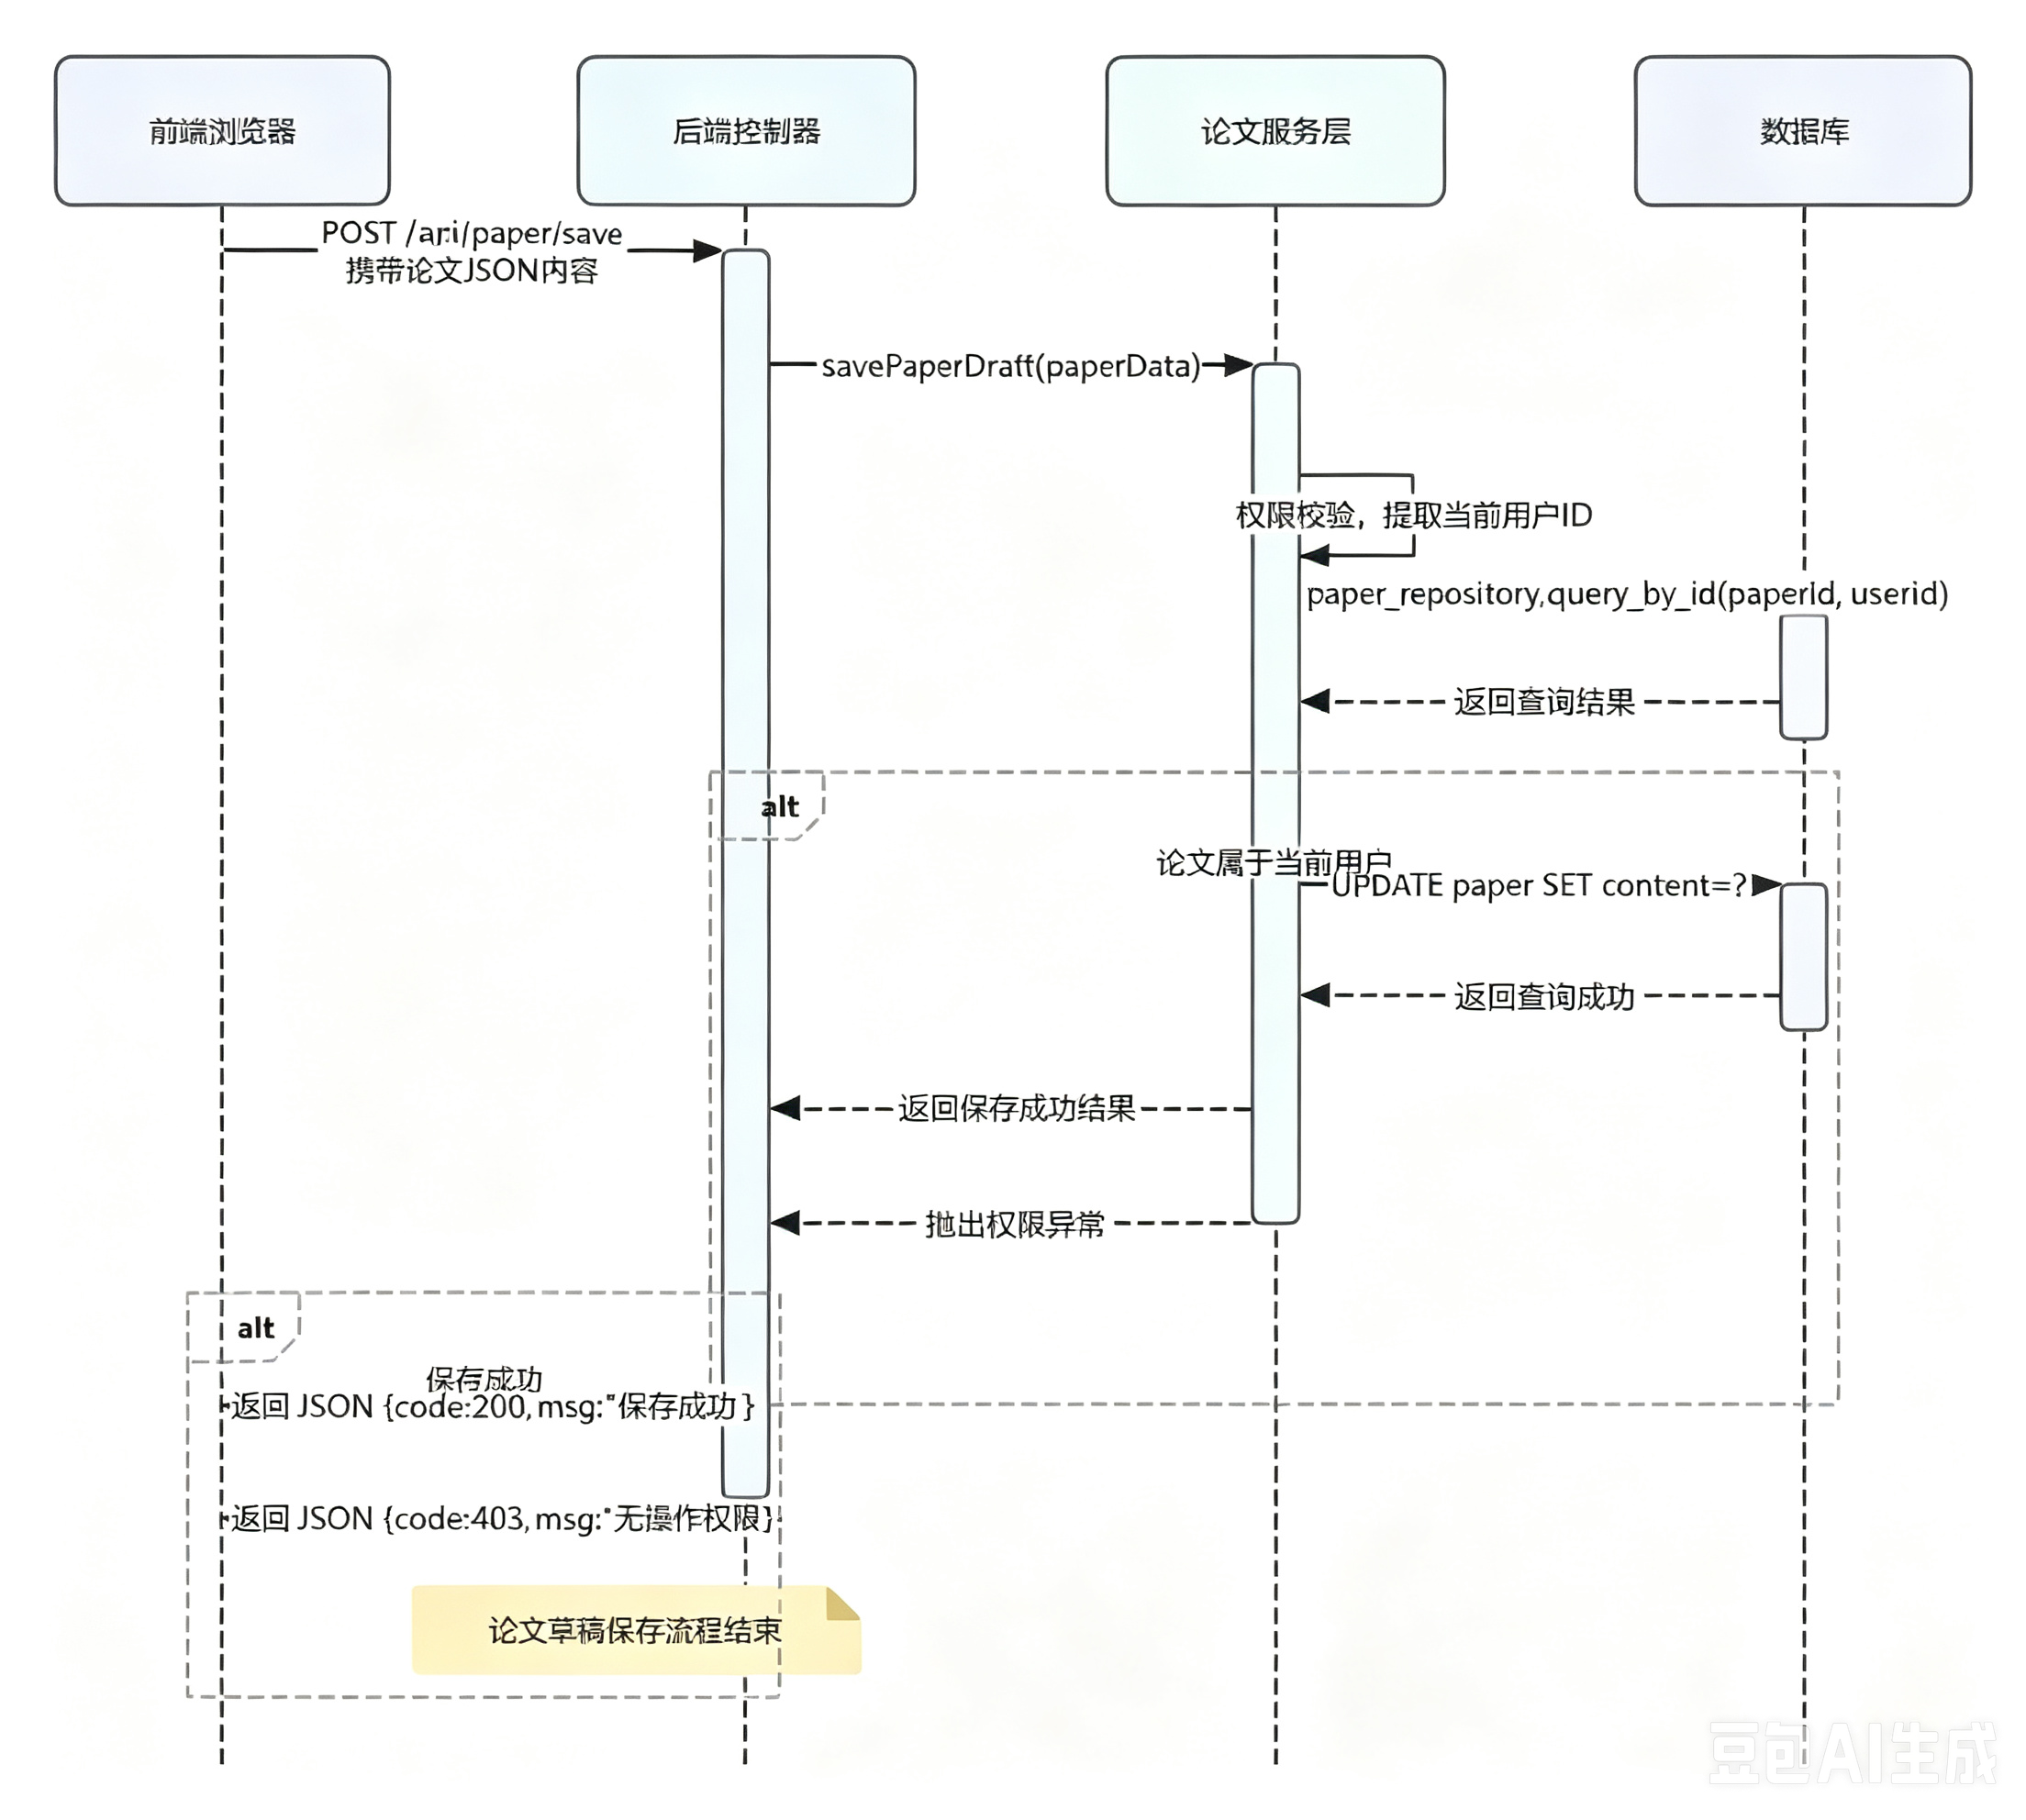
\includegraphics[width=0.9\textwidth]{sequence_diagram.png}
    \caption{论文草稿创建与保存业务时序图}
    \label{fig:seq_diagram}
\end{figure}

	% 插入架构图
	\begin{figure}[htbp]
		\centering
		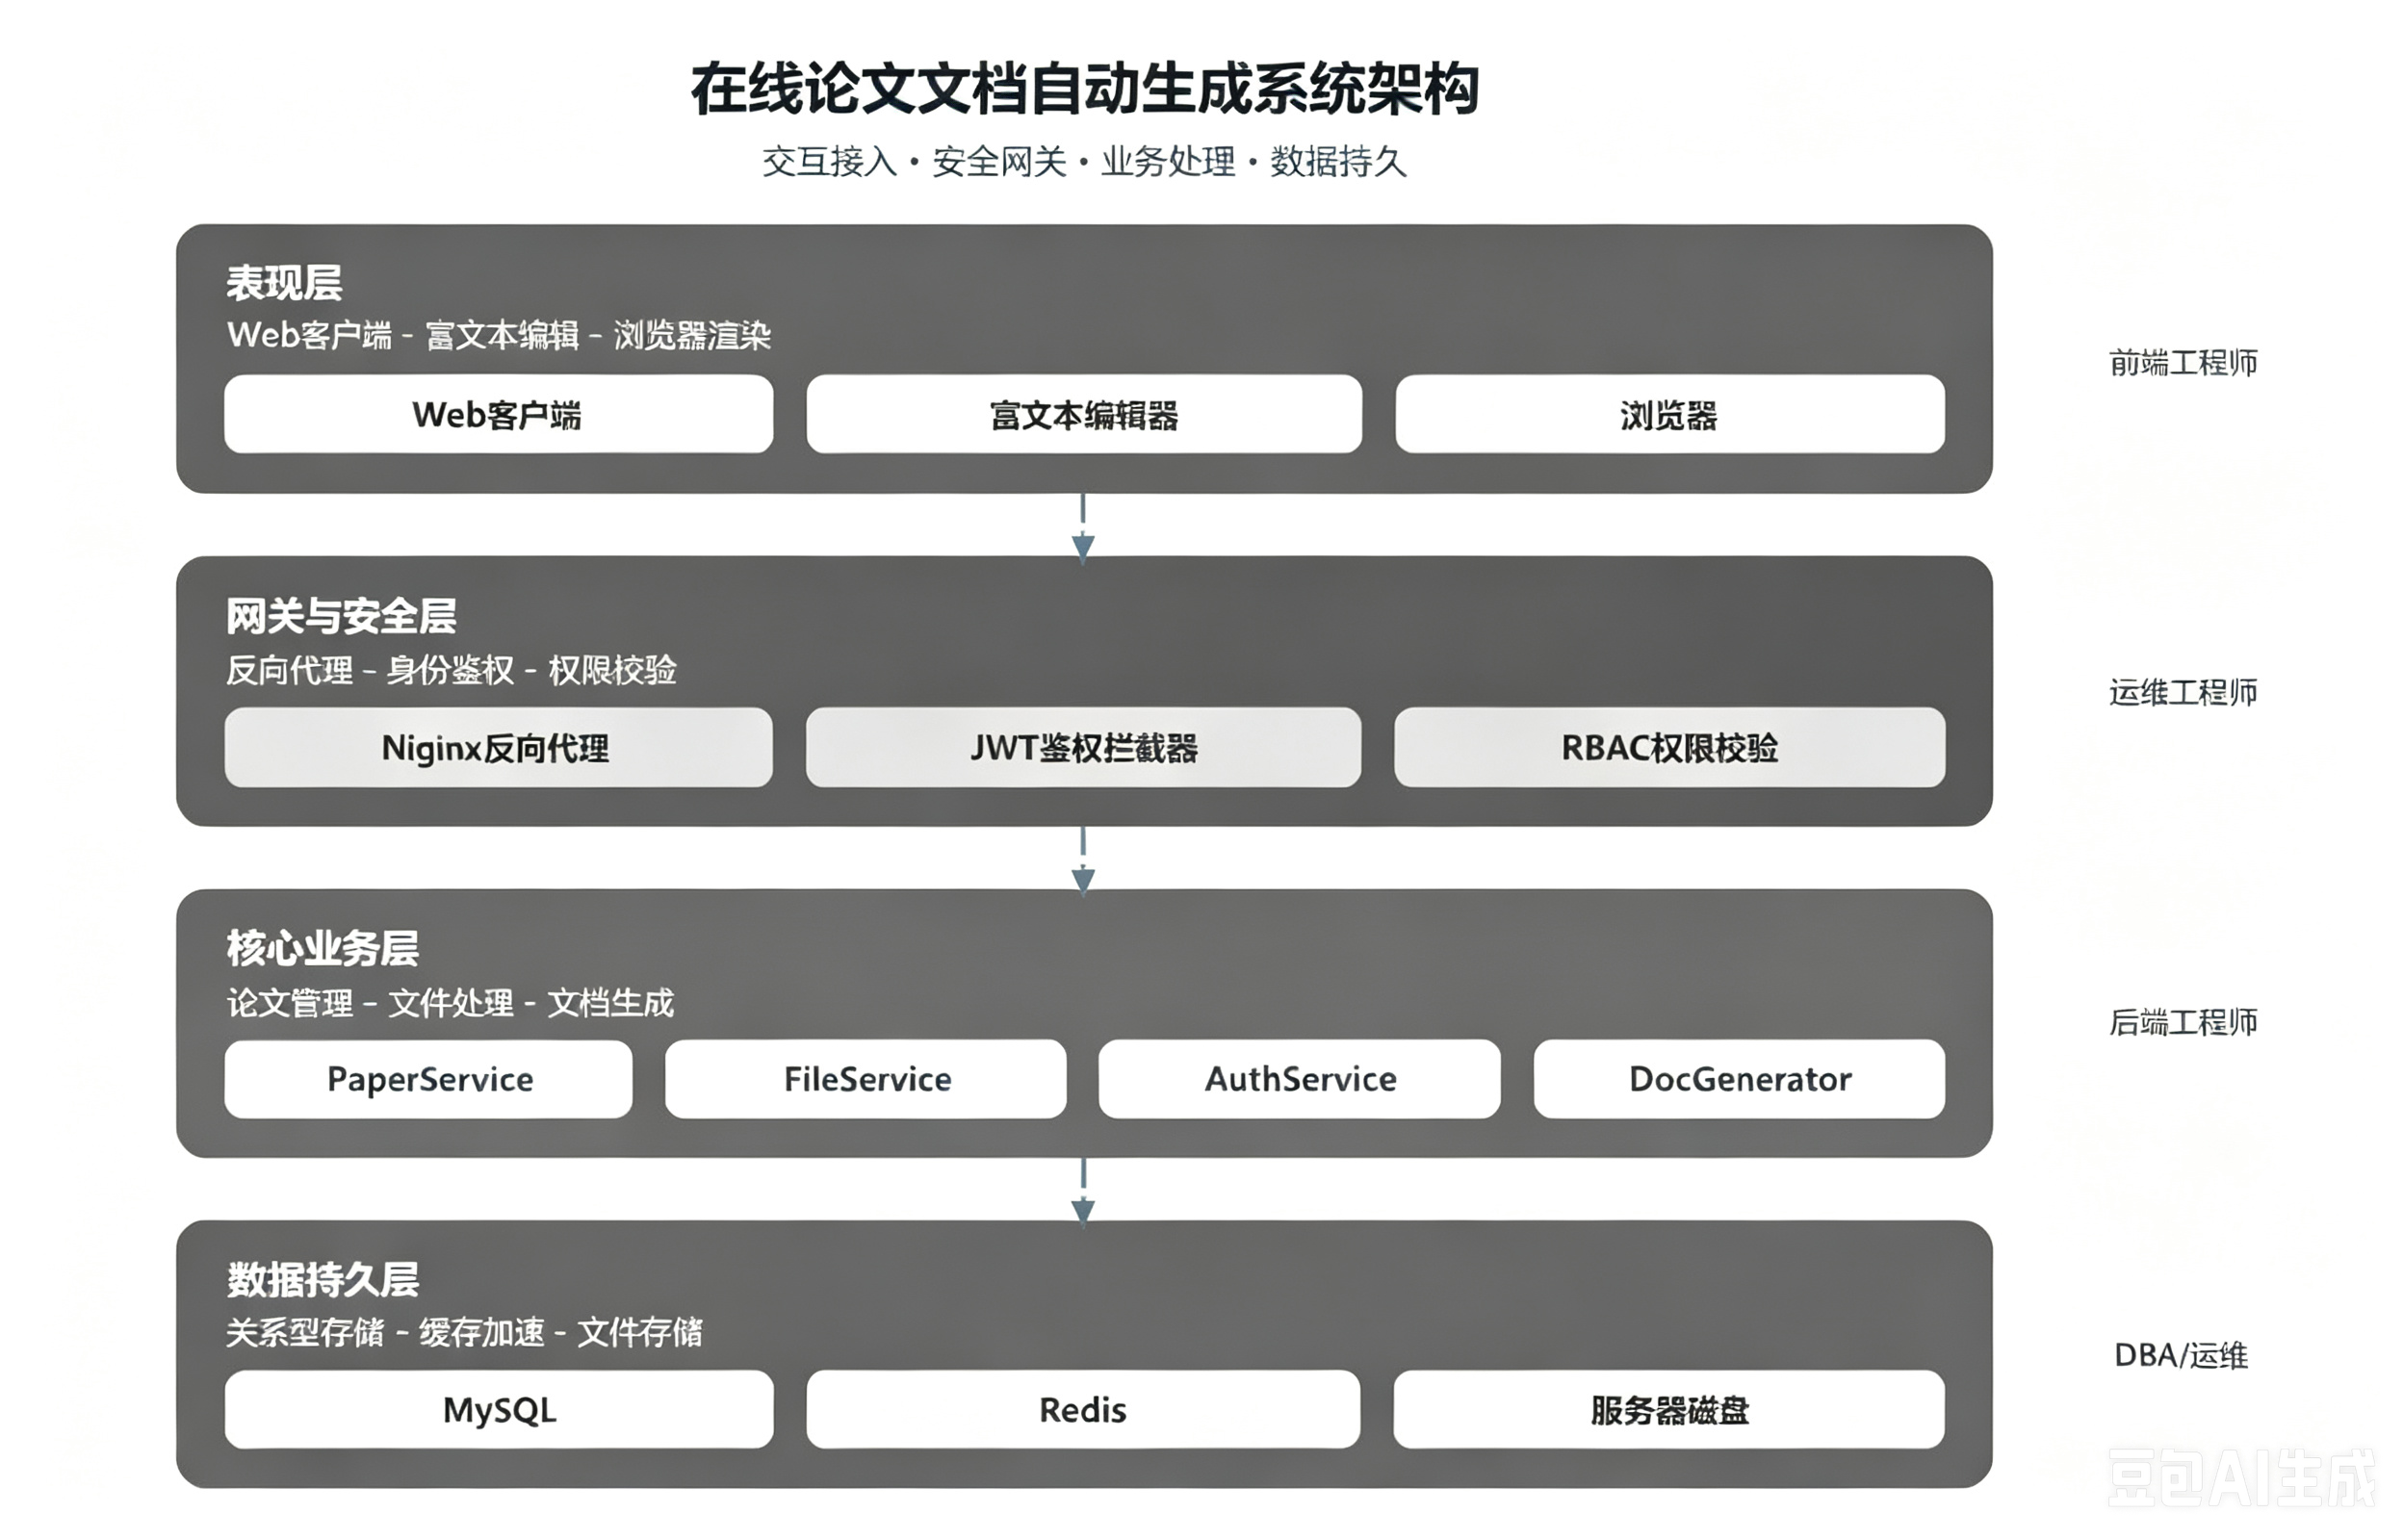
\includegraphics[width=0.95\textwidth]{system_arch.png}
		\caption{在线论文文档自动生成系统详细架构设计图}
		\label{fig:system_arch}
	\end{figure}

	% ------------------------------------------------------------
	\subsection{模块1：用户权限控制模块}

	\subsubsection{模块概述}
	本模块是系统的核心安全中枢，承担全站用户的注册登录、身份凭证分发（JWT签发）、无状态请求拦截验签、以及基于RBAC模型的三类角色权限阻断与放行。本模块为全站提供统一的、基于线程绑定的用户上下文（UserContext）。

	\subsubsection{模块输入输出接口}

	\textbf{（1）用户登录认证接口}：
	\begin{itemize}
		\item \textbf{请求URL}：\texttt{POST /api/auth/login}
		\item \textbf{请求Payload (JSON)}：
	\end{itemize}
	\begin{verbatim}
		{
			"username": "202611001",
			"password": "mypassword123"
		}
	\end{verbatim}
	\begin{itemize}
		\item \textbf{返回Data (JSON)}：
	\end{itemize}
	\begin{verbatim}
		{
			"code": 200,
			"message": "Login Success",
			"data": {
				"token": "eyJhbGciOiJIUzI1NiIsInR5cCI6IkpXVCJ9...",
				"expireTime": 1783932400,
				"userId": 10021,
				"realName": "张同学",
				"role": "STUDENT"
			}
		}
	\end{verbatim}

	\textbf{（2）用户注册接口}：
	\begin{itemize}
		\item \textbf{请求URL}：\texttt{POST /api/auth/register}
		\item \textbf{请求Payload}：
	\end{itemize}
	\begin{verbatim}
		{
			"username": "student01",
			"password": "123456",
			"email": "student01@example.com",
			"realName": "张同学",
			"collegeId": 1,
			"role": "STUDENT"
		}
	\end{verbatim}

	\textbf{（3）Token刷新接口}：
	\begin{itemize}
		\item \textbf{请求URL}：\texttt{POST /api/auth/refresh}
		\item \textbf{请求Header}：\texttt{Authorization: Bearer <Token>}
		\item \textbf{返回Data}：新的JWT Token
	\end{itemize}

	\textbf{（4）用户登出接口}：
	\begin{itemize}
		\item \textbf{请求URL}：\texttt{POST /api/auth/logout}
		\item \textbf{请求Header}：\texttt{Authorization: Bearer <Token>}
		\item \textbf{功能}：将Token加入Redis黑名单
	\end{itemize}

	\subsubsection{模块处理逻辑流程}
	用户访问系统时，基础架构鉴权拦截器的处理逻辑流程如下：
	\begin{enumerate}
		\item 前端发送请求；
		\item 拦截器判断是否为免鉴权白名单（如\texttt{/api/auth/login}、\texttt{/api/auth/register}）；
		\item 若是则直接放行；若否则从请求头提取\texttt{Authorization}；
		\item 解析并验证JWT签名与失效时间；
		\item 检查Redis黑名单是否存在该Token；
		\item 解析对应角色，匹配当前路由访问权限；
		\item 成功后写入运行期线程上下文（Security Context）并放行至后续业务控制器；
		\item 请求结束后清除线程上下文。
	\end{enumerate}

	\subsubsection{权限拦截器的设计细则与扩展性}
	为了满足不同角色在特定业务节点的权限校验需求，设计了基于"声明式注解"的权限控制体系。核心逻辑如下：
	\begin{enumerate}
		\item \textbf{注解扫描}：控制器方法通过\texttt{@RequiresRole(Role.STUDENT)}进行权限标注；
		\item \textbf{前置解析}：权限拦截器通过反射扫描Controller方法上是否存在权限控制注解；
		\item \textbf{逻辑比对}：提取注解中的权限等级与当前上下文中用户的\texttt{role\_code}进行逻辑匹配；
		\item \textbf{扩展说明}：该设计支持权限动态扩展，未来增加"评审组长"或"系主任"角色时，仅需更新枚举类，无需修改拦截器代码，实现高内聚低耦合。
	\end{enumerate}

	\subsubsection{模块内部数据结构}
	\begin{verbatim}
		public class User {
			private Long id;
			private String username;
			private String password;    // BCrypt加密
			private String role;        // ADMIN / STUDENT / TEACHER
			private String realName;
			private String email;
			private Long collegeId;
			private Integer status;     // 1-启用, 0-禁用
			private LocalDateTime createdAt;
			private LocalDateTime updatedAt;
		}
	\end{verbatim}

	\subsubsection{模块算法设计}
	模块核心的"全局请求鉴权过滤算法"在后文"第6节 算法详细设计"中统一展开实现。

	\subsubsection{模块异常处理逻辑}
	\begin{itemize}
		\item Token缺失或无效：抛出401 UnauthenticatedException，返回"未认证，请重新登录"；
		\item Token已过期：抛出401 TokenExpiredException，返回"Token已过期"；
		\item Token在黑名单中：抛出401 TokenBlacklistedException，返回"Token已失效"；
		\item 角色权限不足：抛出403 UnauthorizedException，返回"权限不足"；
		\item 账号已禁用：抛出403 AccountDisabledException，返回"账号已被禁用"。
	\end{itemize}

	% ------------------------------------------------------------
	\subsection{模块2：模板管理模块}

	\subsubsection{模块概述}
	本模块负责学院信息管理和论文模板的完整生命周期管理，包括模板的创建、编辑、版本控制、启用/停用。管理员可通过本模块统一配置论文的章节结构和排版参数，确保全校论文格式规范统一。

	\subsubsection{模块输入输出接口}

	\textbf{（1）创建模板接口}：
	\begin{itemize}
		\item \textbf{请求URL}：\texttt{POST /api/admin/templates}
		\item \textbf{请求Payload (JSON)}：
	\end{itemize}
	\begin{verbatim}
		{
			"name": "本科毕业论文模板",
			"type": "THESIS",
			"collegeId": 1,
			"chapters": [
			"封面", "原创声明", "中文摘要", "英文摘要",
			"第1章 绪论", "第2章 相关理论基础",
			"第3章 系统分析与设计", "第4章 系统实现",
			"第5章 系统测试", "第6章 总结与展望",
			"参考文献", "致谢", "附录"
			],
			"style": {
				"font": "宋体",
				"fontSize": 12,
				"lineSpacing": 1.5,
				"marginLeft": 2.5,
				"marginRight": 2.5,
				"marginTop": 2.5,
				"marginBottom": 2.5,
				"headerFont": "黑体",
				"titleFontSize": 16
			}
		}
	\end{verbatim}

	\textbf{（2）获取模板列表接口}：
	\begin{itemize}
		\item \textbf{请求URL}：\texttt{GET /api/admin/templates}
		\item \textbf{请求参数}：\texttt{page=1\&size=10\&type=THESIS\&collegeId=1}
		\item \textbf{返回Data}：分页模板列表
	\end{itemize}

	\textbf{（3）获取模板详情接口}：
	\begin{itemize}
		\item \textbf{请求URL}：\texttt{GET /api/admin/templates/\{id\}}
		\item \textbf{返回Data}：模板完整信息（含章节结构和排版参数）
	\end{itemize}

	\textbf{（4）更新模板接口}：
	\begin{itemize}
		\item \textbf{请求URL}：\texttt{PUT /api/admin/templates/\{id\}}
		\item \textbf{请求Payload}：同创建模板（版本号自动递增）
	\end{itemize}

	\textbf{（5）启用/停用模板接口}：
	\begin{itemize}
		\item \textbf{请求URL}：\texttt{PATCH /api/admin/templates/\{id\}/status}
		\item \textbf{请求Payload}：\texttt{\{"status": "ENABLED"\}} 或 \texttt{\{"status": "DISABLED"\}}
	\end{itemize}

	\textbf{（6）删除模板接口}：
	\begin{itemize}
		\item \textbf{请求URL}：\texttt{DELETE /api/admin/templates/\{id\}}
		\item \textbf{校验}：模板下已有论文引用时禁止删除
	\end{itemize}

	\textbf{（7）学院管理接口}：
	\begin{itemize}
		\item \texttt{GET /api/admin/colleges}：获取学院列表
		\item \texttt{POST /api/admin/colleges}：创建学院
		\item \texttt{PUT /api/admin/colleges/\{id\}}：更新学院
		\item \texttt{DELETE /api/admin/colleges/\{id\}}：删除学院（需校验无关联模板）
	\end{itemize}

	\subsubsection{模块处理逻辑流程}
	\begin{enumerate}
		\item 管理员登录，JWT验证通过；
		\item 管理员填写模板名称、类型、归属学院；
		\item 管理员配置章节结构（可增删改章节、调整顺序）；
		\item 管理员配置排版参数（字体、字号、行距、页边距等）；
		\item 系统保存模板，初始版本号为V1.0；
		\item 管理员编辑模板时，版本号自动递增（V1.0 → V1.1）；
		\item 管理员可启用或停用模板（停用后学生不可选用，已使用该模板的论文不受影响）；
		\item 模板更新后，学生新建论文自动套用最新版本；
		\item 管理员可在线预览模板效果。
	\end{enumerate}

	\subsubsection{模块内部数据结构}
	\begin{verbatim}
		public class Template {
			private Long id;
			private String name;          // 模板名称
			private String type;          // THESIS / COURSE / PROJECT
			private Long collegeId;
			private String config;        // JSON格式排版参数
			private String chapters;      // JSON格式章节列表
			private String version;       // V1.0, V1.1...
			private String status;        // ENABLED / DISABLED
			private Long createdBy;
			private LocalDateTime createdAt;
			private LocalDateTime updatedAt;
		}

		public class College {
			private Long id;
			private String name;
			private String code;          // 学院编码
			private Integer status;       // 1-启用, 0-停用
			private LocalDateTime createdAt;
			private LocalDateTime updatedAt;
		}
	\end{verbatim}

	\subsubsection{模块算法设计}
	\textbf{版本号递增算法}：
	\begin{enumerate}
		\item 解析当前版本号（如V1.0）；
		\item 提取主版本号和次版本号；
		\item 次版本号+1（V1.0 → V1.1）；
		\item 若次版本号达到10，则主版本号+1，次版本号归零（V1.9 → V2.0）。
	\end{enumerate}

	\subsubsection{模块异常处理逻辑}
	\begin{itemize}
		\item 模板名称重复：抛出400 DuplicateTemplateException，提示"模板名称已存在"；
		\item 模板不存在：抛出404 TemplateNotFoundException，提示"模板不存在"；
		\item 停用模板时已有论文引用：提示"该模板已被论文使用，确认停用？"；
		\item 删除模板时已有论文引用：提示"该模板已被论文使用，无法删除"；
		\item 学院已被模板引用：提示"该学院下存在模板，无法删除"。
	\end{itemize}

	% ------------------------------------------------------------
	\subsection{模块3：论文编辑模块}

	\subsubsection{模块概述}
	本模块是学生端的核心功能，负责基于富文本编辑器的在线论文撰写。学生可根据模板创建论文项目，按章节填写内容，支持图片上传、表格插入、草稿自动保存等完整编辑功能。

	\subsubsection{模块输入输出接口}

	\textbf{（1）创建论文接口}：
	\begin{itemize}
		\item \textbf{请求URL}：\texttt{POST /api/student/papers}
		\item \textbf{请求Payload}：
	\end{itemize}
	\begin{verbatim}
		{
			"templateId": 1,
			"title": "基于Spring Boot的论文管理系统设计与实现"
		}
	\end{verbatim}
	\begin{itemize}
		\item \textbf{返回Data}：\texttt{\{"paperId": 1001\}}
	\end{itemize}

	\textbf{（2）获取论文详情接口}：
	\begin{itemize}
		\item \textbf{请求URL}：\texttt{GET /api/student/papers/\{id\}}
		\item \textbf{返回Data}：
	\end{itemize}
	\begin{verbatim}
		{
			"id": 1001,
			"title": "基于Spring Boot的论文管理系统设计与实现",
			"templateId": 1,
			"status": "DRAFT",
			"chapters": [
			{"id": 1, "title": "绪论", "content": "<p>内容...</p>", "order": 1},
			{"id": 2, "title": "相关技术", "content": "<p>内容...</p>", "order": 2}
			],
			"createdAt": "2026-07-16 10:00:00",
			"updatedAt": "2026-07-16 14:30:00"
		}
	\end{verbatim}

	\textbf{（3）保存论文内容接口}：
	\begin{itemize}
		\item \textbf{请求URL}：\texttt{PUT /api/student/papers/\{id\}}
		\item \textbf{请求Payload}：
	\end{itemize}
	\begin{verbatim}
		{
			"title": "更新后的论文标题",
			"chapters": [
			{"id": 1, "title": "绪论", "content": "<p>更新后的内容...</p>", "order": 1}
			]
		}
	\end{verbatim}

	\textbf{（4）上传图片接口}：
	\begin{itemize}
		\item \textbf{请求URL}：\texttt{POST /api/student/papers/\{id\}/images}
		\item \textbf{请求Payload}：multipart/form-data（图片文件）
		\item \textbf{限制}：JPG、PNG、GIF、SVG格式，最大5MB
		\item \textbf{返回Data}：\texttt{\{"url": "/uploads/images/2026/07/16/xxx.jpg", "id": 101\}}
	\end{itemize}

	\textbf{（5）删除图片接口}：
	\begin{itemize}
		\item \textbf{请求URL}：\texttt{DELETE /api/student/papers/\{id\}/images/\{imageId\}}
	\end{itemize}

	\textbf{（6）获取论文列表接口}：
	\begin{itemize}
		\item \textbf{请求URL}：\texttt{GET /api/student/papers}
		\item \textbf{请求参数}：\texttt{status=DRAFT\&page=1\&size=10}
		\item \textbf{返回Data}：分页论文列表
	\end{itemize}

	\subsubsection{模块处理逻辑流程}
	\begin{enumerate}
		\item 学生登录，JWT验证通过；
		\item 学生选择模板，创建论文项目；
		\item 系统根据模板章节结构自动生成章节大纲；
		\item 学生点击章节，在富文本编辑器中填写内容；
		\item 学生上传图片，插入到指定位置（支持缩放和对齐调整）；
		\item 学生插入表格（支持合并拆分单元格、调整列宽行高）；
		\item 系统每30秒自动保存草稿（内容变化时触发）；
		\item 学生可手动保存（Ctrl+S快捷键）；
		\item 学生可随时切换章节，内容自动保存；
		\item 系统记录论文修改历史（版本号递增）。
	\end{enumerate}

	\subsubsection{模块内部数据结构}
	\begin{verbatim}
		public class Paper {
			private Long id;
			private String title;
			private Long templateId;
			private Long studentId;
			private String content;       // JSON格式章节内容
			private String status;        // DRAFT / SUBMITTED / REVIEWING / APPROVED / REJECTED
			private Integer version;      // 版本号（冲突检测用）
			private LocalDateTime createdAt;
			private LocalDateTime updatedAt;
		}

		public class Chapter {
			private Long id;
			private Long paperId;
			private String title;
			private String content;       // HTML格式富文本内容
			private Integer order;
			private LocalDateTime createdAt;
			private LocalDateTime updatedAt;
		}

		public class PaperImage {
			private Long id;
			private Long paperId;
			private String url;           // 图片存储路径
			private String originalName;  // 原始文件名
			private Long fileSize;        // 文件大小（字节）
			private LocalDateTime uploadedAt;
		}
	\end{verbatim}

	\subsubsection{模块算法设计}
	\textbf{自动保存算法}：
	\begin{enumerate}
		\item 前端定时器每30秒触发一次；
		\item 比对当前内容与上次保存的内容；
		\item 若有变化，发送保存请求；
		\item 若未变化，跳过本次保存；
		\item 保存成功后更新"上次保存内容"副本。
	\end{enumerate}

	\subsubsection{模块异常处理逻辑}
	\begin{itemize}
		\item 保存失败：提示"保存失败，请重试"，保留本地内容；
		\item 图片格式不支持：提示"仅支持JPG、PNG、GIF、SVG格式"；
		\item 图片大小超限：提示"图片大小不能超过5MB"；
		\item 并发冲突：提示"内容已被他人修改，请刷新后重试"；
		\item 论文不存在：返回404。
	\end{itemize}

	% ------------------------------------------------------------
	\subsection{模块4：参考文献管理模块}

	\subsubsection{模块概述}
	本模块负责参考文献的录入、存储、按GB/T 7714标准自动排版、正文引用标注关联。学生可在编辑过程中随时录入文献，系统自动生成标准格式的参考文献列表。

	\subsubsection{模块输入输出接口}

	\textbf{（1）录入参考文献接口}：
	\begin{itemize}
		\item \textbf{请求URL}：\texttt{POST /api/student/papers/\{id\}/references}
		\item \textbf{请求Payload}：
	\end{itemize}
	\begin{verbatim}
		{
			"author": "张三",
			"title": "基于Web的论文管理系统研究",
			"journal": "计算机工程与应用",
			"year": "2026",
			"volume": "42",
			"issue": "3",
			"pages": "45-52",
			"doi": "10.1234/5678",
			"type": "J"
		}
	\end{verbatim}
	\begin{itemize}
		\item \textbf{type说明}：J-期刊，M-专著，D-学位论文，C-会议论文，N-报纸
	\end{itemize}

	\textbf{（2）获取参考文献列表接口}：
	\begin{itemize}
		\item \textbf{请求URL}：\texttt{GET /api/student/papers/\{id\}/references}
		\item \textbf{返回Data}：参考文献列表（已按GB/T 7714格式化）
	\end{itemize}

	\textbf{（3）更新参考文献接口}：
	\begin{itemize}
		\item \textbf{请求URL}：\texttt{PUT /api/student/papers/\{id\}/references/\{refId\}}
		\item \textbf{请求Payload}：同录入接口
	\end{itemize}

	\textbf{（4）删除参考文献接口}：
	\begin{itemize}
		\item \textbf{请求URL}：\texttt{DELETE /api/student/papers/\{id\}/references/\{refId\}}
	\end{itemize}

	\textbf{（5）插入引用标注接口}：
	\begin{itemize}
		\item \textbf{请求URL}：\texttt{POST /api/student/papers/\{id\}/citations}
		\item \textbf{请求Payload}：
	\end{itemize}
	\begin{verbatim}
		{
			"referenceId": 5,
			"position": "chapter-2-3"  // 正文中的引用位置
		}
	\end{verbatim}

	\subsubsection{模块处理逻辑流程}
	\begin{enumerate}
		\item 学生在编辑页面点击"添加参考文献"；
		\item 弹出文献录入表单，逐条填写文献信息；
		\item 系统根据GB/T 7714标准自动生成引用格式；
		\item 学生在正文中标记引用位置（选中文字 → 点击"插入引用"）；
		\item 系统自动生成引用标注序号（如[1]、[2]）；
		\item 参考文献列表按引用顺序排列；
		\item 导出文档时自动生成标准参考文献页。
	\end{enumerate}

	\subsubsection{模块内部数据结构}
	\begin{verbatim}
		public class Reference {
			private Long id;
			private Long paperId;
			private String author;        // 作者
			private String title;         // 题名
			private String journal;       // 刊名
			private String year;          // 年份
			private String volume;        // 卷号
			private String issue;         // 期号
			private String pages;         // 页码
			private String doi;           // DOI号
			private String publisher;     // 出版社（专著用）
			private String address;       // 出版地（专著用）
			private String university;    // 保存单位（学位论文用）
			private String type;          // J / M / D / C / N
			private Integer order;        // 引用序号
			private LocalDateTime createdAt;
			private LocalDateTime updatedAt;
		}

		public class Citation {
			private Long id;
			private Long paperId;
			private Long referenceId;
			private String position;      // 引用位置标识
			private LocalDateTime createdAt;
		}
	\end{verbatim}

	\subsubsection{GB/T 7714格式生成规则与示例}
	\begin{itemize}
		\item \textbf{期刊论文[J]}：作者. 题名[J]. 刊名, 年, 卷(期): 页码.
	\end{itemize}
	\begin{verbatim}
		例：张三. 基于Web的论文管理系统研究[J]. 计算机工程与应用, 2026, 42(3): 45-52.
	\end{verbatim}
	\begin{itemize}
		\item \textbf{专著[M]}：作者. 书名[M]. 出版地: 出版社, 出版年.
	\end{itemize}
	\begin{verbatim}
		例：李四. 软件工程导论[M]. 北京: 清华大学出版社, 2025.
	\end{verbatim}
	\begin{itemize}
		\item \textbf{学位论文[D]}：作者. 题名[D]. 保存地点: 保存单位, 年份.
	\end{itemize}
	\begin{verbatim}
		例：王五. 基于深度学习的文本分类研究[D]. 北京: 北京大学, 2026.
	\end{verbatim}
	\begin{itemize}
		\item \textbf{会议论文[C]}：作者. 题名[C]. 会议名称, 年份, 页码.
	\end{itemize}
	\begin{verbatim}
		例：赵六. 面向大规模数据的快速聚类算法[C]. 中国计算机大会, 2026: 112-118.
	\end{verbatim}

	\subsubsection{模块异常处理逻辑}
	\begin{itemize}
		\item 文献信息不完整：提示"请填写必填字段（作者、题名）"；
		\item 重复引用：提示"该文献已存在，请勿重复录入"；
		\item 参考文献超过200条：提示"参考文献数量已达上限"；
		\item 引用位置无效：提示"请选择正文中的有效位置"。
	\end{itemize}

	% ------------------------------------------------------------
	\subsection{模块5：文档导出模块}

	\subsubsection{模块概述}
	本模块负责网页全文预览、docx格式Word文档导出、PDF格式文档导出。导出时严格按照模板定义的排版参数生成，确保格式一致性。

	\subsubsection{模块输入输出接口}

	\textbf{（1）网页预览接口}：
	\begin{itemize}
		\item \textbf{请求URL}：\texttt{GET /api/student/papers/\{id\}/preview}
		\item \textbf{返回}：完整的HTML页面（模拟A4纸样式）
		\item \textbf{参数}：支持分页浏览
	\end{itemize}

	\textbf{（2）导出Word接口}：
	\begin{itemize}
		\item \textbf{请求URL}：\texttt{GET /api/student/papers/\{id\}/export/docx}
		\item \textbf{返回}：docx文件流（Content-Type: application/vnd.openxmlformats-officedocument.wordprocessingml.document）
		\item \textbf{参数}：\texttt{?scope=full}（整篇）或\texttt{?scope=body}（仅正文）
	\end{itemize}

	\textbf{（3）导出PDF接口}：
	\begin{itemize}
		\item \textbf{请求URL}：\texttt{GET /api/student/papers/\{id\}/export/pdf}
		\item \textbf{返回}：PDF文件流（Content-Type: application/pdf）
		\item \textbf{参数}：\texttt{?scope=full}（整篇）或\texttt{?scope=body}（仅正文）
	\end{itemize}

	\textbf{（4）导出任务状态查询接口}：
	\begin{itemize}
		\item \textbf{请求URL}：\texttt{GET /api/student/papers/export/task/\{taskId\}}
		\item \textbf{返回}：任务状态（PENDING/PROCESSING/COMPLETED/FAILED）
	\end{itemize}

	\subsubsection{模块处理逻辑流程}
	\begin{enumerate}
		\item 学生点击"全文预览"；
		\item 后端组装论文完整内容（封面、原创声明、中英文摘要、正文、参考文献、致谢、附录）；
		\item 应用模板排版参数（字体、字号、行距、页边距等）；
		\item 返回HTML格式预览页面（分页展示）；
		\item 学生点击"导出Word"；
		\item 后端异步生成docx文件（使用Apache POI）；
		\item 学生点击"导出PDF"；
		\item 后端异步生成PDF文件（使用iText）；
		\item 导出完成后提供文件下载链接；
		\item 系统记录导出操作日志。
	\end{enumerate}

	\subsubsection{模块内部数据结构}
	\begin{verbatim}
		public class ExportTask {
			private Long id;
			private Long paperId;
			private Long userId;
			private String format;       // DOCX / PDF
			private String scope;        // FULL / BODY
			private String status;       // PENDING / PROCESSING / COMPLETED / FAILED
			private String filePath;
			private Long fileSize;
			private String errorMessage;
			private LocalDateTime createdAt;
			private LocalDateTime completedAt;
		}
	\end{verbatim}

	\subsubsection{模块算法设计}
	\textbf{Word生成算法（Apache POI）}：
	\begin{enumerate}
		\item 创建XWPFDocument对象；
		\item 根据模板配置设置页面边距（CTPageMar）；
		\item 生成封面页（标题、姓名、学号、学院、日期）；
		\item 生成原创声明页；
		\item 生成中英文摘要页；
		\item 生成目录（自动提取标题层级）；
		\item 生成正文（遍历章节，应用样式：标题1/标题2/正文）；
		\item 嵌入图片（XWPFRun.addPicture）；
		\item 生成参考文献列表；
		\item 生成致谢和附录；
		\item 保存文档到临时目录；
		\item 返回文件流。
	\end{enumerate}

	\textbf{PDF生成算法（iText）}：
	\begin{enumerate}
		\item 创建Document对象（PageSize.A4）；
		\item 设置页面边距；
		\item 添加封面内容（PdfPTable布局）；
		\item 添加正文内容（逐章节渲染）；
		\item 渲染图片（Image对象）；
		\item 渲染表格（PdfPTable）；
		\item 添加参考文献；
		\item 关闭文档，输出PDF；
		\item 返回文件流。
	\end{enumerate}

	\subsubsection{模块异常处理逻辑}
	\begin{itemize}
		\item 导出失败：记录错误日志，提示"导出失败，请稍后重试"；
		\item 导出超时（超过60秒）：提示"导出任务超时，请稍后重试"；
		\item 文件不存在：返回404；
		\item 论文内容为空：提示"论文内容为空，请先编辑内容"；
		\item 图片加载失败：跳过该图片，记录日志。
	\end{itemize}

	% ------------------------------------------------------------
	\subsection{模块6：批阅管理模块}

	\subsubsection{模块概述}
	本模块负责课程论文的提交、在线批阅、批注添加、评语评分、退回修改、历史版本记录。教师可在线查看学生论文，在任意位置添加批注，填写整体评语并评定分数和等级。

	\subsubsection{模块输入输出接口}

	\textbf{（1）提交论文接口}：
	\begin{itemize}
		\item \textbf{请求URL}：\texttt{POST /api/student/papers/\{id\}/submit}
		\item \textbf{请求Payload}：无
		\item \textbf{校验}：论文状态须为DRAFT，内容不能为空
		\item \textbf{返回}：提交成功提示，论文状态变更为SUBMITTED
	\end{itemize}

	\textbf{（2）获取待批阅列表接口（教师）}：
	\begin{itemize}
		\item \textbf{请求URL}：\texttt{GET /api/teacher/papers/submitted}
		\item \textbf{请求参数}：\texttt{page=1\&size=10}
		\item \textbf{返回Data}：已提交论文列表（含学生信息）
	\end{itemize}

	\textbf{（3）获取论文详情（教师批阅视图）}：
	\begin{itemize}
		\item \textbf{请求URL}：\texttt{GET /api/teacher/papers/\{id\}}
		\item \textbf{返回Data}：论文完整内容（只读模式）
	\end{itemize}

	\textbf{（4）添加批注接口}：
	\begin{itemize}
		\item \textbf{请求URL}：\texttt{POST /api/teacher/papers/\{id\}/annotations}
		\item \textbf{请求Payload}：
	\end{itemize}
	\begin{verbatim}
		{
			"position": "chapter-2-3",      // 标识批注位置
			"content": "这一段需要补充数据支撑",
			"startOffset": 45,              // 起始偏移量
			"endOffset": 128                // 结束偏移量
		}
	\end{verbatim}

	\textbf{（5）更新批注接口}：
	\begin{itemize}
		\item \textbf{请求URL}：\texttt{PUT /api/teacher/papers/\{id\}/annotations/\{annotationId\}}
		\item \textbf{请求Payload}：\texttt{\{"content": "更新后的批注内容"\}}
	\end{itemize}

	\textbf{（6）删除批注接口}：
	\begin{itemize}
		\item \textbf{请求URL}：\texttt{DELETE /api/teacher/papers/\{id\}/annotations/\{annotationId\}}
	\end{itemize}

	\textbf{（7）提交评阅意见接口}：
	\begin{itemize}
		\item \textbf{请求URL}：\texttt{POST /api/teacher/papers/\{id\}/review}
		\item \textbf{请求Payload}：
	\end{itemize}
	\begin{verbatim}
		{
			"score": 85.5,
			"grade": "良好",
			"comment": "论文结构清晰，论证充分，但实验数据略显不足。建议补充更多对比实验。",
			"action": "REJECT"              // APPROVE / REJECT
		}
	\end{verbatim}
	\begin{itemize}
		\item \textbf{校验}：action为REJECT时，comment不能为空
	\end{itemize}

	\textbf{（8）获取批阅历史接口}：
	\begin{itemize}
		\item \textbf{请求URL}：\texttt{GET /api/teacher/papers/\{id\}/history}
		\item \textbf{返回Data}：批阅历史列表（含版本、操作人、操作时间、操作类型）
	\end{itemize}

	\textbf{（9）学生查看批阅结果接口}：
	\begin{itemize}
		\item \textbf{请求URL}：\texttt{GET /api/student/papers/\{id\}/review}
		\item \textbf{返回Data}：批注列表、评语、分数、等级、批阅状态
	\end{itemize}

	\subsubsection{模块处理逻辑流程}
	\begin{enumerate}
		\item 学生完成论文编辑后点击"提交批阅"；
		\item 系统验证论文内容不为空、无必填项缺失；
		\item 系统锁定文档，状态变更为"已提交（SUBMITTED）"；
		\item 教师登录，查看待批阅列表；
		\item 教师选择论文，进入批阅视图（只读模式）；
		\item 教师阅读论文，在指定位置添加批注（选中文字→添加批注）；
		\item 批注以高亮标记显示在论文中；
		\item 教师填写整体评语、评定分数和等级；
		\item 教师点击"通过（APPROVE）"或"退回（REJECT）"；
		\item 若为退回，强制填写修改意见；
		\item 退回后论文状态变更为"已退回（REJECTED）"，文档解锁；
		\item 学生收到通知，查看批注和修改意见；
		\item 学生修改后重新提交，进入下一轮批阅；
		\item 若为通过，论文状态变更为"已通过（APPROVED）"；
		\item 系统留存每一次提交、批阅、退回的版本记录。
	\end{enumerate}

	\subsubsection{模块内部数据结构}
	\begin{verbatim}
		public class Review {
			private Long id;
			private Long paperId;
			private Long reviewerId;         // 教师ID
			private String comment;          // 整体评语
			private String annotations;      // JSON格式批注列表
			private Double score;
			private String grade;            // 优秀/良好/中等/及格/不及格
			private String action;           // APPROVE / REJECT
			private Integer version;
			private LocalDateTime createdAt;
			private LocalDateTime updatedAt;
		}

		public class Annotation {
			private Long id;
			private Long paperId;
			private Long reviewId;
			private String position;         // 位置标识
			private Integer startOffset;     // 起始偏移量
			private Integer endOffset;       // 结束偏移量
			private String content;          // 批注内容
			private String status;           // ACTIVE / RESOLVED
			private LocalDateTime createdAt;
			private LocalDateTime updatedAt;
		}

		public class VersionHistory {
			private Long id;
			private Long paperId;
			private String contentSnapshot;  // 论文快照
			private String action;           // SUBMIT / REJECT / APPROVE
			private Long operatorId;
			private String operatorName;
			private LocalDateTime createdAt;
		}

		public class ReviewStatus {
			public static final String DRAFT = "DRAFT";
			public static final String SUBMITTED = "SUBMITTED";
			public static final String REVIEWING = "REVIEWING";
			public static final String APPROVED = "APPROVED";
			public static final String REJECTED = "REJECTED";
		}
	\end{verbatim}

	\subsubsection{模块算法设计}
	\textbf{版本记录算法}：
	\begin{enumerate}
		\item 每次提交时保存当前论文完整内容的快照；
		\item 生成版本号（V1, V2, V3...）；
		\item 记录操作类型（SUBMIT/REJECT/APPROVE）；
		\item 记录操作人ID和操作时间；
		\item 历史记录按时间倒序排列。
	\end{enumerate}

	\textbf{状态流转规则}：
	\begin{verbatim}
		DRAFT → SUBMITTED → REVIEWING → APPROVED (通过)
		↓
		REJECTED (退回) → DRAFT → SUBMITTED → ...
	\end{verbatim}

	\subsubsection{模块异常处理逻辑}
	\begin{itemize}
		\item 重复提交：提示"论文已提交，等待批阅"；
		\item 已锁定论文不可编辑：提示"论文已提交，不可编辑"；
		\item 教师权限不足：抛出403 UnauthorizedException；
		\item 批注内容为空：提示"批注内容不能为空"；
		\item 分数超出范围：提示"分数应在0-100之间"；
		\item 退回时未填写修改意见：提示"请填写修改意见"。
	\end{itemize}


	% ============================================================
	\section{接口详细设计}

	\subsection{外部接口详细设计}

	\subsubsection{用户交互接口}
	采用基于HTTP/1.1的Web可视化人机交互界面，页面输入参数通过JSON异步传输。所有接口使用UTF-8编码。

	\subsubsection{第三方软件接口}
	\begin{itemize}
		\item 数据库接口：MySQL JDBC驱动，HikariCP连接池；
		\item 文档生成接口：Apache POI 5.x（Word）、iText 7.x（PDF）；
		\item 缓存接口：Redis客户端（Lettuce/Jedis），用于Token黑名单；
		\item 文件存储接口：Java NIO处理上传，存储至本地文件系统。
	\end{itemize}

	\subsubsection{硬件接口}
	无专用硬件外设接口，依赖标准网络协议（TCP/IP）和服务器基础资源（CPU、内存、磁盘）。

	\subsection{内部模块接口详细设计}

	\subsubsection{模块间请求参数定义}
	所有受保护的业务接口，前端在发起HTTP请求时，必须在Header中强制注入：
	\begin{verbatim}
		Authorization: Bearer <Token_String>
		Content-Type: application/json
	\end{verbatim}

	\subsubsection{返回数据结构定义}
	统一返回对象封装结构：
	\begin{verbatim}
		{
			"code": 200,
			"message": "success",
			"data": {...}
		}
	\end{verbatim}

	\subsubsection{核心业务接口契约表}
	\begin{table}[htbp]
		\centering
		\caption{核心业务接口契约表}
		\begin{tabular}{|p{3.5cm}|p{2cm}|p{5cm}|}
			\hline
			\textbf{接口名称} & \textbf{方法} & \textbf{关键参数与校验规则} \\
			\hline
			论文内容保存 & PUT & paper\_id(Long, 必填), content(String, 最大64KB) \\
			\hline
			用户登录认证 & POST & username(3-20位), password(6-20位) \\
			\hline
			模板资源加载 & GET & college\_id(Long), 需校验用户所属学院 \\
			\hline
			论文分数录入 & POST & paper\_id, score(0-100), 仅教师角色调用 \\
			\hline
			参考文献录入 & POST & paper\_id, author, title(必填) \\
			\hline
			文档导出 & GET & paper\_id, scope(FULL/BODY) \\
			\hline
			批注添加 & POST & paper\_id, position, content(最大500字符) \\
			\hline
		\end{tabular}
	\end{table}

	\subsubsection{调用时序说明}
	调用链由基础架构网关/拦截器优先触发，验签成功并解出用户上下文后，生命周期才移交给具体的业务子模块，最终返回JSON响应。


	% ============================================================
	\section{数据结构详细设计}

	% 插入E-R图（保留）
	\begin{figure}[htbp]
		\centering
		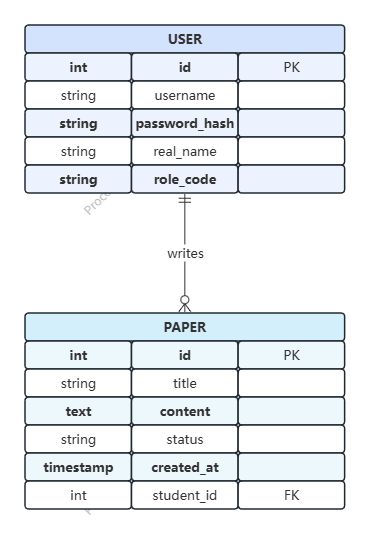
\includegraphics[width=0.85\textwidth]{database_er.png}
		\caption{系统核心业务数据实体关系（E-R）图}
		\label{fig:database_er}
	\end{figure}

	\subsection{全局数据结构说明}
	系统在运行期通过ThreadLocal绑定当前请求线程的用户上下文，实现全流程用户身份的无感知传递。

	\subsubsection{线程上下文结构}
	\begin{verbatim}
		public class UserContext {
			private static ThreadLocal<UserContext> context = new ThreadLocal<>();
			private Long userId;
			private String username;
			private String role;
			private Long collegeId;
			private String clientIp;

			// getter/setter 方法
			public static UserContext getCurrent() { return context.get(); }
			public static void setCurrent(UserContext ctx) { context.set(ctx); }
			public static void clear() { context.remove(); }
		}
	\end{verbatim}

	\subsection{数据库表详细设计}
	采用MySQL 8.0关系型数据库，由基础架构统一设计并建立以下系统核心表：

	\subsubsection{用户主表 (sys\_user)}
	存储系统所有管理员、教师、学生账号的安全凭证及属性。
	\begin{table}[htbp]
		\centering
		\begin{tabular}{|l|l|l|l|l|}
			\hline
			\textbf{字段名} & \textbf{数据类型} & \textbf{可空} & \textbf{默认值} & \textbf{说明与约束} \\
			\hline
			id & bigint & NO & 自增 & 主键ID \\
			username & varchar(32) & NO & 无 & UNIQUE, 登录账号 \\
			password & varchar(128) & NO & 无 & BCrypt加密密文 \\
			role & varchar(20) & NO & 无 & ADMIN/STUDENT/TEACHER \\
			real\_name & varchar(32) & NO & 无 & 真实姓名 \\
			email & varchar(100) & NO & 无 & 邮箱 \\
			college\_id & bigint & YES & NULL & 所属学院ID \\
			status & tinyint & NO & 1 & 1-启用, 0-禁用 \\
			created\_at & datetime & NO & CURRENT\_TIMESTAMP & 创建时间 \\
			updated\_at & datetime & NO & CURRENT\_TIMESTAMP & 更新时间 \\
			\hline
		\end{tabular}
		\caption{用户表结构}
	\end{table}

	\textbf{索引设计}：
	\begin{itemize}
		\item PRIMARY KEY (id)：聚集索引；
		\item UNIQUE INDEX uk\_username (username)：保障账号唯一；
		\item INDEX idx\_college\_role (college\_id, role)：便于分学院管理。
	\end{itemize}

	\subsubsection{学院信息表 (sys\_college)}
	\begin{table}[htbp]
		\centering
		\begin{tabular}{|l|l|l|l|l|}
			\hline
			\textbf{字段名} & \textbf{数据类型} & \textbf{可空} & \textbf{默认值} & \textbf{说明与约束} \\
			\hline
			id & bigint & NO & 自增 & 学院主键ID \\
			college\_name & varchar(64) & NO & 无 & UNIQUE, 院系全称 \\
			code & varchar(20) & NO & 无 & UNIQUE, 学院编码 \\
			status & tinyint & NO & 1 & 1-启用, 0-停用 \\
			created\_at & datetime & NO & CURRENT\_TIMESTAMP & 创建时间 \\
			updated\_at & datetime & NO & CURRENT\_TIMESTAMP & 更新时间 \\
			\hline
		\end{tabular}
		\caption{学院表结构}
	\end{table}

	\subsubsection{模板表 (tmpl\_template)}
	\begin{table}[htbp]
		\centering
		\begin{tabular}{|l|l|l|l|l|}
			\hline
			\textbf{字段名} & \textbf{数据类型} & \textbf{可空} & \textbf{默认值} & \textbf{说明与约束} \\
			\hline
			id & bigint & NO & 自增 & 模板主键ID \\
			name & varchar(200) & NO & 无 & 模板名称 \\
			type & varchar(20) & NO & 无 & THESIS/COURSE/PROJECT \\
			college\_id & bigint & YES & NULL & 所属学院ID \\
			config & json & NO & 无 & 排版参数 \\
			chapters & json & NO & 无 & 章节结构 \\
			version & varchar(20) & NO & V1.0 & 版本号 \\
			status & varchar(20) & NO & ENABLED & ENABLED/DISABLED \\
			created\_by & bigint & NO & 无 & 创建人ID \\
			created\_at & datetime & NO & CURRENT\_TIMESTAMP & 创建时间 \\
			updated\_at & datetime & NO & CURRENT\_TIMESTAMP & 更新时间 \\
			\hline
		\end{tabular}
		\caption{模板表结构}
	\end{table}

	\subsubsection{论文主表 (paper\_main)}
	\begin{table}[htbp]
		\centering
		\begin{tabular}{|l|l|l|l|l|}
			\hline
			\textbf{字段名} & \textbf{数据类型} & \textbf{可空} & \textbf{默认值} & \textbf{说明与约束} \\
			\hline
			id & bigint & NO & 自增 & 论文主键ID \\
			title & varchar(500) & NO & 无 & 论文标题 \\
			template\_id & bigint & YES & NULL & 模板ID \\
			student\_id & bigint & NO & 无 & 学生ID \\
			teacher\_id & bigint & YES & NULL & 教师ID \\
			content & json & YES & NULL & 章节内容 \\
			status & varchar(20) & NO & DRAFT & DRAFT/SUBMITTED/REVIEWING/APPROVED/REJECTED \\
			version & int & NO & 1 & 乐观锁版本号 \\
			created\_at & datetime & NO & CURRENT\_TIMESTAMP & 创建时间 \\
			updated\_at & datetime & NO & CURRENT\_TIMESTAMP & 更新时间 \\
			\hline
		\end{tabular}
		\caption{论文表结构}
	\end{table}

	\subsubsection{参考文献表 (paper\_reference)}
	\begin{table}[htbp]
		\centering
		\begin{tabular}{|l|l|l|l|l|}
			\hline
			\textbf{字段名} & \textbf{数据类型} & \textbf{可空} & \textbf{默认值} & \textbf{说明与约束} \\
			\hline
			id & bigint & NO & 自增 & 文献主键ID \\
			paper\_id & bigint & NO & 无 & 论文ID \\
			author & varchar(200) & YES & NULL & 作者 \\
			title & varchar(500) & NO & 无 & 题名 \\
			journal & varchar(200) & YES & NULL & 刊名 \\
			year & varchar(20) & YES & NULL & 年份 \\
			volume & varchar(20) & YES & NULL & 卷号 \\
			issue & varchar(20) & YES & NULL & 期号 \\
			pages & varchar(50) & YES & NULL & 页码 \\
			doi & varchar(100) & YES & NULL & DOI号 \\
			type & varchar(10) & NO & J & J/M/D/C/N \\
			order\_num & int & YES & NULL & 引用序号 \\
			created\_at & datetime & NO & CURRENT\_TIMESTAMP & 创建时间 \\
			updated\_at & datetime & NO & CURRENT\_TIMESTAMP & 更新时间 \\
			\hline
		\end{tabular}
		\caption{参考文献表结构}
	\end{table}

	\subsubsection{批阅记录表 (review\_record)}
	\begin{table}[htbp]
		\centering
		\begin{tabular}{|l|l|l|l|l|}
			\hline
			\textbf{字段名} & \textbf{数据类型} & \textbf{可空} & \textbf{默认值} & \textbf{说明与约束} \\
			\hline
			id & bigint & NO & 自增 & 批阅记录ID \\
			paper\_id & bigint & NO & 无 & 论文ID \\
			reviewer\_id & bigint & NO & 无 & 教师ID \\
			comment & text & YES & NULL & 整体评语 \\
			annotations & json & YES & NULL & 批注列表 \\
			score & decimal(5,2) & YES & NULL & 分数(0-100) \\
			grade & varchar(20) & YES & NULL & 优秀/良好/中等/及格/不及格 \\
			action & varchar(20) & NO & 无 & APPROVE/REJECT \\
			version & int & NO & 1 & 版本号 \\
			created\_at & datetime & NO & CURRENT\_TIMESTAMP & 创建时间 \\
			updated\_at & datetime & NO & CURRENT\_TIMESTAMP & 更新时间 \\
			\hline
		\end{tabular}
		\caption{批阅记录表结构}
	\end{table}

	\subsubsection{版本历史表 (version\_history)}
	\begin{table}[htbp]
		\centering
		\begin{tabular}{|l|l|l|l|l|}
			\hline
			\textbf{字段名} & \textbf{数据类型} & \textbf{可空} & \textbf{默认值} & \textbf{说明与约束} \\
			\hline
			id & bigint & NO & 自增 & 历史记录ID \\
			paper\_id & bigint & NO & 无 & 论文ID \\
			content\_snapshot & json & YES & NULL & 论文快照 \\
			action & varchar(20) & NO & 无 & SUBMIT/REJECT/APPROVE \\
			operator\_id & bigint & NO & 无 & 操作人ID \\
			operator\_name & varchar(50) & YES & NULL & 操作人姓名 \\
			created\_at & datetime & NO & CURRENT\_TIMESTAMP & 操作时间 \\
			\hline
		\end{tabular}
		\caption{版本历史表结构}
	\end{table}

	\subsection{缓存/临时数据结构设计}
	\begin{itemize}
		\item \textbf{Token黑名单}：Redis存储，Key: \texttt{auth:blacklist:token:\{md5(token)\}}，TTL为Token剩余有效期；
		\item \textbf{临时导出文件}：存储在服务器临时目录（/tmp/export/），导出完成后30分钟自动清理；
		\item \textbf{用户会话上下文}：ThreadLocal存储，请求结束后自动清除；
		\item \textbf{论文草稿缓存}：Redis存储，Key: \texttt{draft:paper:\{paperId\}:user:\{userId\}}，TTL为7天。
	\end{itemize}


	% ============================================================
	\section{算法详细设计}

	\subsection{核心算法1：全局请求鉴权与RBAC隔离算法}

	\subsubsection{算法描述}
	拦截器对进入系统的HTTP请求执行动态路由拆包、合法性验签、时效性检查，并严格依据路由前缀实施多角色垂直越权拦截，成功后将用户实体封装挂载至线程上下文。

	\subsubsection{输入输出参数}
	\begin{itemize}
		\item \textbf{输入}：HttpServletRequest（包含请求头及RequestURI）
		\item \textbf{输出}：boolean（True放行，False拒绝）
	\end{itemize}

	\subsubsection{伪代码实现}
	\begin{verbatim}
		function preHandle(request, response):
		// 1. 路由白名单直接放行（登录/注册）
		if request.uri starts with "/api/auth/":
		return true

		// 2. 从Header提取Token
		authHeader = request.getHeader("Authorization")
		if authHeader is null or not starts with "Bearer ":
		throw UnauthenticatedException("Missing token")
		token = authHeader.substring(7)

		// 3. 检查Redis黑名单
		if redis.exists("auth:blacklist:token:" + md5(token)):
		throw UnauthenticatedException("Token blacklisted")

		// 4. 解析验证JWT
		payload = JwtUtil.parseToken(token)
		if payload is null or payload.isExpired():
		throw UnauthenticatedException("Token expired")

		// 5. RBAC垂直越权拦截
		role = payload.getRole()
		uri = request.getRequestURI()
		if uri starts with "/api/admin/" and role != "ADMIN":
		throw UnauthorizedException("Admin only")
		if uri starts with "/api/teacher/" and role not in ["TEACHER", "ADMIN"]:
		throw UnauthorizedException("Teacher only")
		if uri starts with "/api/student/" and role not in ["STUDENT", "TEACHER", "ADMIN"]:
		throw UnauthorizedException("Student only")

		// 6. 写入线程上下文
		UserContext.set(payload.userId, payload.username, role, payload.collegeId)
		return true
	\end{verbatim}

	\subsubsection{边界条件处理}
	\begin{itemize}
		\item Token过期：前端自动跳转登录页，提示"登录已过期，请重新登录"；
		\item Token黑名单：Redis中检测到则拒绝，提示"Token已失效"；
		\item 并发请求Token刚过期：Refresh Token机制静默刷新，用户无感知；
		\item 请求头缺失：返回401，提示"未提供认证凭证"。
	\end{itemize}

	% ------------------------------------------------------------
	\subsection{核心算法2：论文草稿冲突检测算法}

	考虑到多端协同编辑场景（用户可能同时在多个设备或浏览器标签页中打开同一篇论文），基础架构引入了乐观锁版本号锁定算法，确保数据一致性：

	\begin{enumerate}
		\item \textbf{锁定检查}：用户打开论文草稿时，获取当前数据库记录的\texttt{version}值并缓存到前端；
		\item \textbf{提交核验}：保存内容时，SQL语句执行：
	\end{enumerate}
	\begin{verbatim}
		UPDATE paper
		SET content = ?, version = version + 1, updated_at = NOW()
		WHERE id = ? AND version = ?
	\end{verbatim}
	\begin{enumerate}
		\setcounter{enumi}{2}
		\item \textbf{冲突处理}：若执行影响行数为0，说明数据已被他人修改，系统抛出\texttt{DataVersionConflictException}，返回错误码409，强制前端刷新并提示用户合并内容。
	\end{enumerate}

	\begin{verbatim}
		function savePaper(paperId, newContent, expectedVersion):
		// 1. 查询当前论文
		current = paperRepository.findById(paperId)
		if current is null:
		throw NotFoundException("Paper not found")

		// 2. 检查版本号
		if current.version != expectedVersion:
		throw ConflictException("内容已被他人修改，请刷新后重试")

		// 3. 更新数据
		current.content = newContent
		current.version = expectedVersion + 1
		current.updatedAt = now()
		paperRepository.save(current)

		return current
	\end{verbatim}

	% ------------------------------------------------------------
	\subsection{核心算法3：参考文献自动排版（GB/T 7714）}

	\subsubsection{算法描述}
	根据GB/T 7714-2015标准，将文献信息转换为标准引用格式字符串。系统支持期刊论文（J）、专著（M）、学位论文（D）、会议论文（C）、报纸（N）五种常见文献类型。

	\subsubsection{输入输出参数}
	\begin{itemize}
		\item \textbf{输入}：Reference对象（作者、题名、刊名、年份、卷号、期号、页码、类型）
		\item \textbf{输出}：符合GB/T 7714标准的格式化字符串
	\end{itemize}

	\subsubsection{伪代码实现}
	\begin{verbatim}
		function formatReference(ref):
		// 1. 处理作者（多个作者用逗号分隔）
		authors = ref.author.split(",")
		if authors.length > 3:
		formattedAuthors = authors[0] + ", " + authors[1] + ", " + authors[2] + ", 等"
		else:
		formattedAuthors = authors.join(", ")

		// 2. 构建引用字符串
		result = formattedAuthors + ". "
		result += ref.title

		// 3. 根据类型生成不同格式
		switch ref.type:
		case "J":   // 期刊
		result += "[J]. " + ref.journal + ", "
		result += ref.year + ", " + ref.volume
		if ref.issue is not null:
		result += "(" + ref.issue + ")"
		result += ": " + ref.pages + "."
		case "M":   // 专著
		result += "[M]. " + ref.publisher + ", " + ref.year + "."
		case "D":   // 学位论文
		result += "[D]. " + ref.university + ", " + ref.year + "."
		case "C":   // 会议论文
		result += "[C]. " + ref.conference + ", " + ref.year + ": " + ref.pages + "."
		case "N":   // 报纸
		result += "[N]. " + ref.newspaper + ", " + ref.date + "(" + ref.edition + ")."

		return result
	\end{verbatim}

	\subsubsection{格式示例}
	\begin{verbatim}
		期刊论文：张三. 基于Web的论文管理系统研究[J]. 计算机工程与应用, 2026, 42(3): 45-52.
		专著：李四. 软件工程导论[M]. 北京: 清华大学出版社, 2025.
		学位论文：王五. 基于深度学习的文本分类研究[D]. 北京: 北京大学, 2026.
	\end{verbatim}

	\subsubsection{边界条件处理}
	\begin{itemize}
		\item 作者为空：使用"佚名"；
		\item 年份为空：使用"n.d."（无日期）；
		\item 页码为空：使用空字符串；
		\item 超过3个作者：使用"等"缩写。
	\end{itemize}

	% ------------------------------------------------------------
	\subsection{核心算法4：Word文档生成算法}

	\subsubsection{算法描述}
	使用Apache POI库将论文数据转换为符合模板排版规范的标准Word文档（docx格式）。

	\subsubsection{伪代码实现}
	\begin{verbatim}
		function generateWord(paper, template):
		// 1. 创建文档
		doc = new XWPFDocument()

		// 2. 设置页面
		setPageMargins(doc, template.style)

		// 3. 生成封面
		generateCover(doc, paper, template)

		// 4. 生成原创声明
		generateDeclaration(doc)

		// 5. 生成摘要
		generateAbstract(doc, paper)

		// 6. 生成目录
		generateTOC(doc)

		// 7. 生成正文
		for each chapter in paper.chapters:
		generateChapter(doc, chapter, template.style)

		// 8. 生成参考文献
		generateReferences(doc, paper.references)

		// 9. 生成致谢
		generateAcknowledgement(doc)

		// 10. 保存并返回
		return doc.getBytes()
	\end{verbatim}

	\subsubsection{性能优化策略}
	\begin{itemize}
		\item 大文档处理：采用流式写入，避免内存溢出；
		\item 图片处理：自动压缩图片至合适分辨率；
		\item 缓存机制：模板样式缓存，避免重复解析。
	\end{itemize}


	% ============================================================
	\section{界面详细设计}

	\subsection{页面1：登录/注册页面}

	\subsubsection{页面布局与控件说明}
	\begin{itemize}
		\item 居中卡片式布局，背景为渐变或纯色；
		\item 标题区：系统Logo和名称；
		\item 表单区：用户名输入框、密码输入框（登录模式）/ 用户名、密码、确认密码、邮箱、真实姓名（注册模式）；
		\item 操作区：登录/注册按钮；
		\item 切换区：登录/注册模式切换链接；
		\item 密码框支持显示/隐藏密码切换。
	\end{itemize}

	\subsubsection{页面交互逻辑}
	\begin{itemize}
		\item 登录模式默认显示，点击"去注册"切换到注册模式；
		\item 注册成功后自动切换到登录模式并清空密码；
		\item 登录成功后跳转到论文编辑页面；
		\item 输入框支持回车键提交；
		\item 表单校验实时反馈。
	\end{itemize}

	\subsubsection{页面输入校验规则}
	\begin{itemize}
		\item 用户名：3-20位字符，字母数字组合；
		\item 密码：6-30位字符；
		\item 确认密码：与密码一致；
		\item 邮箱：符合邮箱格式；
		\item 真实姓名：2-20位中文字符；
		\item 禁用SQL注入关键字（select、drop、--等）。
	\end{itemize}

	% ------------------------------------------------------------
	\subsection{页面2：论文编辑页面}

	\subsubsection{页面布局与控件说明}
	\begin{itemize}
		\item 顶部：论文标题输入框、保存按钮、预览按钮、提交按钮；
		\item 左侧：章节大纲列表（显示所有章节，支持点击切换、添加、删除、重命名、拖拽排序）；
		\item 中间：富文本编辑器（TipTap），包含工具栏（加粗、斜体、标题、对齐、列表、图片、表格、引用、代码块）和编辑区；
		\item 右侧：参考文献管理面板（文献列表、添加、删除、引用插入）；
		\item 底部：字数统计、自动保存状态（�� 已保存/�� 保存中...）。
	\end{itemize}

	\subsubsection{页面交互逻辑}
	\begin{itemize}
		\item 点击章节大纲切换编辑内容；
		\item 编辑器内容变化后自动触发保存（30秒防抖）；
		\item 点击"保存"手动保存当前内容；
		\item 点击"预览"在新窗口打开全文预览；
		\item 点击"提交"弹出确认对话框，确认后锁定文档；
		\item 支持Ctrl+S快捷键保存。
	\end{itemize}

	\subsubsection{页面输入校验规则}
	\begin{itemize}
		\item 论文标题不能为空，长度不超过500字符；
		\item 章节内容不能为空；
		\item 章节标题不能为空；
		\item 每章节内容不超过50000字。
	\end{itemize}

	% ------------------------------------------------------------
	\subsection{页面3：批阅管理页面（教师端）}

	\subsubsection{页面布局与控件说明}
	\begin{itemize}
		\item 顶部：论文信息（标题、学生姓名、学号、学院、提交时间）；
		\item 左侧：论文内容预览（只读模式，显示完整排版，A4纸样式）；
		\item 右侧：批注面板（点击论文内容位置可添加批注，已添加批注高亮显示，批注列表可展开/折叠）；
		\item 底部：评语输入框、分数输入框（0-100）、等级选择下拉框（优秀/良好/中等/及格/不及格）、通过/退回按钮；
		\item 历史记录按钮：查看全部版本历史。
	\end{itemize}

	\subsubsection{页面交互逻辑}
	\begin{itemize}
		\item 点击论文内容任意位置弹出批注输入框；
		\item 批注以高亮标记显示在论文中；
		\item 批注可编辑和删除；
		\item 填写评语和分数后点击"通过"或"退回"；
		\item 退回时强制填写修改意见；
		\item 查看历史版本可点击"历史记录"按钮；
		\item 支持批量批阅（下一篇/上一篇）。
	\end{itemize}


	% ============================================================

    \section{出错处理详细设计}

\subsection{全局错误码规范}
为了提高前后端对接效率及系统异常的可追溯性，系统定义了统一的全局错误码规范。所有 API 异常响应均遵循以下标准格式：

\begin{table}[htbp]
    \centering
    \caption{全局错误码对照表}
    \begin{tabular}{|p{3cm}|p{4cm}|p{6cm}|}
        \hline
        \textbf{错误码} & \textbf{错误类型} & \textbf{说明} \\
        \hline
        ERR\_AUTH\_001 & Token 失效 & 用户凭证过期或非法，需重新登录 \\
        \hline
        ERR\_AUTH\_002 & 权限不足 & 当前用户角色无权访问该资源 \\
        \hline
        ERR\_DB\_001 & 数据查询失败 & 数据库连接超时或查询语句异常 \\
        \hline
        ERR\_DB\_002 & 数据写入冲突 & 并发操作导致的数据乐观锁冲突 \\
        \hline
        ERR\_PARAM\_001 & 参数校验失败 & 输入格式不符合要求或缺少必填项 \\
        \hline
        ERR\_BIZ\_001 & 业务逻辑异常 & 论文状态不符合当前操作要求 \\
        \hline
        ERR\_SYS\_999 & 系统内部错误 & 未知异常，建议查看后台堆栈日志 \\
        \hline
    \end{tabular}
    \label{tab:error_code}
\end{table}

\subsection{模块内部异常分类}
% 此处接你原有的异常分类内容...

	\subsection{模块内部异常分类}
	\begin{itemize}
		\item \textbf{认证异常（401）}：Token缺失、Token无效、Token过期、Token黑名单；
		\item \textbf{授权异常（403）}：垂直越权、水平越权、账号禁用；
		\item \textbf{业务异常（400）}：参数校验失败、业务规则冲突；
		\item \textbf{资源异常（404）}：论文不存在、模板不存在、用户不存在、参考文献不存在；
		\item \textbf{冲突异常（409）}：数据版本冲突、资源已存在；
		\item \textbf{系统异常（500）}：数据库连接失败、文件读写失败、文档生成失败、图片处理失败。
	\end{itemize}

	\subsection{异常捕获流程}
	任何业务层抛出的异常，均向上抛出并最终由全局异常处理器（GlobalExceptionHandler）统一捕获，封装为标准JSON响应返回前端。

	\subsection{异常返回信息定义}
	\begin{verbatim}
		{
			"code": 403,
			"message": "Access Denied: Illegal privilege escalation detected.",
			"data": null
		}
	\end{verbatim}

	\subsection{全局错误码定义}
	\begin{table}[htbp]
		\centering
		\caption{全局错误码定义}
		\begin{tabular}{|c|c|c|}
			\hline
			\textbf{错误码} & \textbf{类型} & \textbf{说明} \\
			\hline
			200 & SUCCESS & 请求成功 \\
			400 & BAD\_REQUEST & 请求参数错误 \\
			401 & UNAUTHORIZED & 未认证/Token失效 \\
			403 & FORBIDDEN & 权限不足 \\
			404 & NOT\_FOUND & 资源不存在 \\
			409 & CONFLICT & 资源冲突 \\
			500 & SERVER\_ERROR & 服务器内部错误 \\
			503 & SERVICE\_UNAVAILABLE & 服务不可用（导出超时等） \\
			\hline
		\end{tabular}
	\end{table}

	\subsection{异常恢复处理方案}
	\begin{itemize}
		\item 数据库操作：开启事务，异常自动回滚；
		\item 文件操作：删除临时文件，记录日志；
		\item 网络请求：设置超时和重试机制（最多3次）；
		\item 文档导出：异步处理，超时提示重试；
		\item 图片上传：失败时保留用户本地缓存。
	\end{itemize}


	% ============================================================
	\section{安全详细设计}

	\subsection{身份校验逻辑}
	全面实行基于JWT的无状态身份验证，密钥通过环境变量密存，Token设置2小时过期时间，支持Refresh Token机制。

	\subsection{数据加密处理设计}
	\begin{itemize}
		\item 用户密码：BCrypt强哈希加密（工作因子$\ge$10），严禁明文存储；
		\item 传输加密：生产环境启用HTTPS，TLS 1.2及以上；
		\item 敏感配置：使用环境变量，不入Git仓库；
		\item 数据库连接：用户名密码加密存储。
	\end{itemize}

	\subsection{防攻击处理逻辑}
	\begin{enumerate}
		\item \textbf{SQL注入防御}：使用参数化查询（JPA/MyBatis），禁止拼接SQL；
		\item \textbf{XSS防御}：用户输入严格过滤转义，前端输出转义；
		\item \textbf{CSRF防御}：状态变更请求验证CSRF Token；
		\item \textbf{水平越权防御}：所有数据操作必须验证当前用户是否有权操作该数据；
		\item \textbf{垂直越权防御}：拦截器强制校验角色与路由权限匹配；
		\item \textbf{文件上传防御}：校验MIME类型，重命名存储，限制大小。
	\end{enumerate}

	\subsection{水平越权防御代码范式}
	\begin{verbatim}
		// 强制约束：所有数据操作必须验证所有权
		Long currentUserId = SecurityContextHolder.getUserId();
		Paper paper = paperRepository.findById(paperId);
		if (!paper.getStudentId().equals(currentUserId)) {
			throw new UnauthorizedException("无权访问他人论文");
		}
	\end{verbatim}


	% ============================================================
	\section{维护详细设计}

	\subsection{日志模块设计}
	\begin{itemize}
		\item 使用SLF4J + Logback日志框架；
		\item 日志级别：ERROR、WARN、INFO、DEBUG；
		\item 关键操作自动记录审计日志：登录、注册、论文创建/修改/提交、模板管理、批阅操作、文档导出；
		\item 日志格式：时间、级别、类名、方法名、操作内容、操作人ID、IP地址、请求ID；
		\item 日志保留周期：180天；
		\item 日志按日期滚动归档。
	\end{itemize}

	\subsection{配置项设计}
	\begin{table}[htbp]
		\centering
		\caption{核心配置项列表}
		\begin{tabular}{|p{5cm}|p{3cm}|p{3cm}|}
			\hline
			\textbf{配置项} & \textbf{默认值} & \textbf{说明} \\
			\hline
			jwt.secret & - & JWT签名密钥（必填） \\
			jwt.expiration & 7200000 & Token过期时间（毫秒，默认2小时） \\
			spring.datasource.url & - & 数据库连接URL \\
			spring.datasource.username & - & 数据库用户名 \\
			spring.datasource.password & - & 数据库密码 \\
			file.upload-path & ./uploads & 文件上传路径 \\
			spring.servlet.multipart.max-file-size & 5MB & 单文件最大大小 \\
			export.temp-path & /tmp/export & 导出临时文件路径 \\
			export.max-wait-time & 60000 & 导出最大等待时间（毫秒） \\
			logging.level.com.paper & debug & 日志级别 \\
			\hline
		\end{tabular}
	\end{table}

	\subsection{数据备份逻辑}
	\begin{itemize}
		\item 数据库每日凌晨2:00自动全量备份；
		\item 备份保留30天；
		\item 导出文件临时目录每小时自动清理；
		\item 关键操作具备事务性，保证数据一致性；
		\item 论文内容每次保存记录版本号，支持回滚。
	\end{itemize}
    \subsection{部署架构说明}
为了确保系统的高可用性与可维护性，本系统采用基于 Docker 的容器化部署方案。部署架构设计遵循“基础设施即代码”原则：

\begin{itemize}
    \item \textbf{部署环境}：使用 Docker Compose 实现服务编排，将 Web 服务、MySQL 数据库与 Redis 缓存部署在同一隔离的网络桥接层内。
    \item \textbf{持续集成/部署 (CI/CD)}：所有代码变更通过 GitHub Actions 触发自动化构建，生成镜像并推送至私有仓库。
    \item \textbf{流量控制}：前端静态资源与后端 API 统一通过 Nginx 进行反向代理，并配置 Gzip 压缩以优化页面加载性能。
\end{itemize}

% 插入部署架构示意图位置占位
\begin{figure}[htbp]
    \centering
    % \includegraphics[width=0.8\textwidth]{deployment_arch.png}
    \caption{系统容器化部署架构示意图}
    \label{fig:deployment}
\end{figure}
	
	\subsection{系统监控设计}
	为了确保系统在高并发场景下的稳定性，设计了基础架构监控模块：
	\begin{itemize}
		\item \textbf{链路跟踪}：每个HTTP请求分配唯一\texttt{trace\_id}，在系统日志中透传，实现请求的全生命周期追踪；
		\item \textbf{性能统计}：拦截器计算每个业务方法的执行耗时（Execution Time），若超过300ms则记录至慢查询日志；
		\item \textbf{连接池监控}：实时监控数据库连接池的活跃连接数与空闲连接数，预警连接泄漏风险；
		\item \textbf{健康检查}：提供\texttt{/actuator/health}端点，返回系统健康状态；
		\item \textbf{指标暴露}：提供\texttt{/actuator/metrics}端点，暴露系统运行指标。
	\end{itemize}
	
	\subsection{部署与运维}
	\begin{itemize}
		\item 支持Docker容器化部署；
		\item 支持Nginx反向代理和负载均衡；
		\item 支持多环境配置（dev/test/prod）；
		\item 支持日志集中收集（ELK）；
		\item 支持应用监控（Prometheus + Grafana）。
	\end{itemize}
	
\end{document}